\section{Diseño}
\label{section:diseno}

\subsection{Metodología de desarrollo}
\label{sec:metodologia_desarrollo}
Para el desarrollo de la aplicacion se ha utilizado el desarrollo guiado por pruebas de software, o Test-driven development (TDD)[Figura 14]. Sus dos reglas principales son:
\begin{itemize}
 \item Escribir las pruebas primero.
 \item Refactorización.
\end{itemize}

Para escribir las pruebas se utilizaron pruebas unitarias. En primer lugar, se escribe una prueba y se verifica que las pruebas fallan. A continuación, se implementa el código que hace que la prueba pase satisfactoriamente y seguidamente se refactoriza el código escrito. El propósito del desarrollo guiado por pruebas es lograr un código limpio que funcione. La idea es que los requisitos sean traducidos a pruebas, de este modo, cuando las pruebas pasen se garantizará que el software cumple con los requisitos que se han establecido.

Una ventaja de esta forma de programación es el evitar escribir código innecesario. Se intenta escribir el mínimo código posible, y si el código pasa una prueba aunque sepamos que es incorrecto nos da una idea de que tenemos que modificar nuestra lista de requerimientos agregando uno nuevo.

La generación de pruebas para cada funcionalidad hace que el programador confíe en el código escrito. Esto permite hacer modificaciones profundas del código pues sabemos que si luego logramos hacer pasar todas las pruebas tendremos un código que funcione correctamente.

Otra característica del desarrollo guiado por pruebas de software es que requiere que el programador primero haga fallar los casos de prueba. La idea es asegurarse de que los casos de prueba realmente funcionen y puedan recoger un error.

A pesar de los elevados requisitos iniciales de aplicar esta metodología, el desarrollo guiado por pruebas (TDD) puede proporcionar un gran valor añadido en la creación de software, produciendo aplicaciones de más calidad y en menos tiempo. Ofrece más que una simple validación del cumplimiento de los requisitos, también puede guiar el diseño de un programa. Centrándose en primer lugar en los casos de prueba uno debe imaginarse cómo los clientes utilizarán la funcionalidad (en este caso, los casos de prueba). Por lo tanto, al programador solo le importa la interfaz y no la implementación. Esta ventaja es similar al diseño por convenio pero se parece a él por los casos de prueba más que por las aserciones matemáticas.

 \begin{figure}[h]
 \centering
 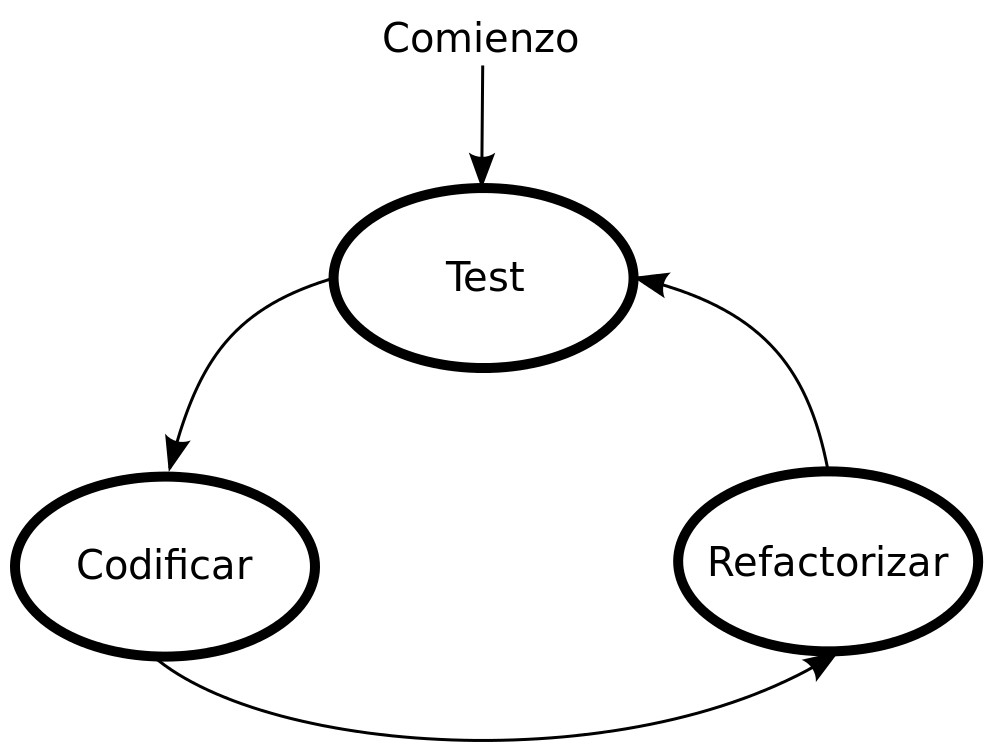
\includegraphics[scale=0.3]{../images/tdd.png}
 \caption{Test-driven development (TDD).}
 \label{fig:../images/tdd.png}
 \end{figure}

\subsection{Tecnología utilizada}
\label{sec:tecnologia_utilizada}
\
Para la codificación de la aplicacion se ha utilizado el Framework de desarrollo Lluvia basado en el lenguaje de programación JavaScript. 

Lluvia es una API Open Source que incorpora gran parte de las funciones nativas de Ruby. Soporta multihilo a pequeña escala y provee de un sistema de mensajería asíncrono gestionado por señales. 

En Lluvia, los Devices son los encargados de proporcionar el mecanismo asincrono de comunicacion. Estan preparados para disparar eventos y recibir mensajes de otros Devices, estos mesajes se almacenan en una cola de mensajes para que sean procesados cuando llege su turno. A efectos practicos, cada Device se comporta como una aplicacion independiente del resto.

Para gestionar los eventos del DOM de HTML se utilizan los Gates de Lluvia que estan capacitados para mantener el campo de visibilidad del objeto. 

La conjunción de los Devices y los Gates proporciona un metodo dinamico y agil para la creacion de la aplicación web. 
\subsection{Clases principales de la aplicación}
\label{sec:clases_principlaes}

\subsubsection{World}
\label{sec:world}
La clase World deriva de Device y es la encargada de generar el mundo donde coexisten los nanobots y speakers. Es necesario indicarle el canvas(elemento HTML incorporado en HMTL5 que permite la generación de gráficos dinámicamente por medio del scripting) donde se realizará la representación gráfica y optativo el ancho y largo del mismo. 

En la clase World se almacena un array con todos los nanobot y speakers que se hayan generado  para su facil manipulacion. Para ir almacenandolos se llama al metodo has\_born() que se encarga de almacenar el nanobot creado y disparar el evento new\_boid.

Dispone de un método run() que es llamado cada cierto tiempo para su ejecución. En él,  se actualiza el tiempo del procesador y se pinta el mundo.

Se dispone del método new\_boid\_of() para crear nuevos boids de la clase que se desee. Para la llamada del método es posible pasarle en los argumentos el tipo de entidad que se quiere crear(boid, nanobot o speaker) y un bloque. En el bloque se puede pasar una configuración inicial de la entidad para darle valores iniciales.

Los métodos visible\_for() y audible\_for() permiten comprobar que se puede ver o escuchar desde determinado lugar del mundo, estos métodos son llamados desde los nanobots o speakers para saber que pueden ver u oír desde su posición. Se consideró que este método era más adecuado integrarlo en el mundo, en vez de en el nanobot o boid, para tener la posibilidad de saber que se puede ver en algún lugar del mundo sin la necesidad de que allí esté situado un nanobot.

La clase World es capaz de atender al evento focus\_boid que se encarga de saber si un nanobot esta resaltado y poder dibujar en pantalla información adicional sobre su velocidad y aceleración.

Por último, dispone de los clásicos métodos para poder acceder de manera segura a distintas variables de la clase.

\subsubsection{Boid}
\label{sec:boid}
La clase Boid es clase padre tanto de Nanobot como de Speaker. Es la encargada de dotarlos de unas propiedades básicas idénticas para ambas clases hijas.
 
Un boid se puede inicializar con un objeto de configuración capaz de sobrescribir todos los  valores por defecto de los atributos.

Se crea un objeto donde se almacena toda la información de la posicion, velocidad y aceleración del boid, este objeto se llama geo\_data. Además, se dota al boid de una masa, color, visión y cerebro por defecto.
 
Se crea un puntero al mundo donde vivirá, especialmente útil para poder utilizar los metodos visible\_for() y audible\_for() de la clase World.

También se crean tres variables que almacenan las fuerzas limites de cada boids: thrust, steering, braking (aceleración, ángulo de giro y frenado).
 
Dispone de un metodo run() que es llamado cada interacción del programa para poder actualizar su aceleración en función de la media de todas las aceleraciones que devuelvan los comportamientos activos, además de, actualizar su tiempo actual.
 
El método clip() se encarga de adecuar la aceleración y velocidad actual para que se cumplan las fuerzas limite de cada boid. Si se pasa de aceleración o velocidad aqui se vuelve al estado anterior de dicha magnitud.
 
Por último, dispone de los clásicos métodos para poder acceder de manera segura a distintas variables de la clase.

\subsubsection{Nanobot}
\label{sec:nanobot}

La clase Nanobot deriva de la clase Boid y es la encargada de crear nuevos nanobot en el mundo.
 
Para su creación es necesario pasarle un bloque de configuración, que este a su vez pasará a la clase padre para asignarle los valores. Además, se crea un nivel de estrés, un radio para la longitud que alcanzara el habla del nanobot, un array de frecuencias donde se almacenarán todas las frecuencias que vaya escuchando el nanobot y un array de objetos visibles.
 
El nanobot es capaz de comunicarse con otros por medio de su método talk(). Para realizar la comunicación se comprueba quien puede escuchar y a esos se les manda un mensaje con set\_msg(). Dicho mensaje se trata de un objeto compuesto por la palabra que se quiere comunicar y un puntero al nanobot emisor. Los mensajes según llegan al receptor se guardan en un array de mensajes para poder leerlos de manera asíncrona y no perder información. A la hora de analizar dichos mensajes, en analyze\_msg(), se comprueba cual es la palabra que se pasa en el mensaje y en función de su contenido se ejecuta unas instrucciones u otras. 

Hay instrucciones que son órdenes que activan comportamientos directamente, para estas es necesario tener un objetivo para el comportamiento, para ello se utiliza el puntero al emisor. A la hora de crear la réplica se elegirá al azar de un array de réplicas que existen para cada caso.
 
El nanobot es capaz de recibir frecuencias, con el metodo set\_frequency(), de una onda de sonido. En el método analyze\_sound() se comprobara el valor de la frecuencia y en funcion de su valor aumentara o disminuirá el nivel de estrés del nanobot.


El método listen() encapsula todo lo relacionado con el sistema auditivo del nanobot.

\subsubsection{Speaker}
\label{sec:speaker}

La clase Speaker deriva de la clase Boid y es la encargada de crear nuevos speakers en el mundo.

Para su creación es necesario pasarle un bloque de configuración, que este a su vez pasará a la clase padre para asignarle los valores. Ademas, se crea un radio para la longitud que tendrá la música que reproduzca el speaker, variables para saber la frecuencia a la que emite, conocer si esta apagado o encendido, así como, para conocer su volumen.

El speaker se podrá encender o apagar con los métodos on() y off(). Si esta apagado la música parará y no se reproducirá nada. Se podra aumentar y disminuir el volumen con los métodos voluemn\_up() y volumen\_down().

La frecuencia a la que emite se puede obtener a traves del metodo set\_frequency\_music() y se podrá mandar a quien escuche con get\_frequency\_music().

\subsubsection{World interface}
\label{sec:world_interface}
La clase World interface deriva de la clase Device y es la gestora de crear el dispositivo encargado de poder seleccionar a los nanobots para poder observar sus características y opciones.

Es capaz de atender el mensaje new\_boid que se encarga de añadir un nuevo nanobot o speaker al dispositivo para su selección. 

\subsubsection{Boid editor}
\label{sec:boid_editor}
La clase Boid editor deriva de Device y es la encargada de mostrar toda la informacion u opciones para el speaker o nanobot que este selecionado en el World\_interface. 

Si se trata de un nanobot mostrara la posicion actual, el comportamiento activo en ese momento y su nivel de estrés. Además, mostrará una serie de controles para el manejo independiente de cada uno de los boids.

Si el seleccionado es un speaker mostrará los controles para manipular el speaker, que son: boton de apagado y encendido, subir y bajar volumen, cambiar cancion y la canción que actualmente se está reproduciendo.  

\subsubsection{Brain}
\label{sec:brain}
La clase Brain es la encargada de gestionar todos los comportamientos que puedan estar asociados a un nanobot y devolver la aceleración ponderada de todas las aceleraciones individuales devueltas por los comportamientos.

Es capaz de activar y desactivar comportamientos con los métodos activate() y deactivate(). Esto ayuda a crear comportamientos más complejos que los inicialmente propuesto gracias a la combinación de comportamientos simples.

También se puede preguntar al cerebro con can\$U() si un comportamiento puede ser activado en un determinado nanobot.

\subsubsection{Beahavior}
\label{sec:beahavior}
La clase Behavior permite modelar el comportamiento de los boids. Esto se consigue modificando el vector de aceleración que cada uno de los boids posee como parte de su estructura interna. Un comportamiento se puede definir como un objeto que devuelve una aceleración deseada en un momento concreto.

Al ser una clase abstracta, no permite crear instancias, de manera que para crear un comportamiento nuevo es necesario generar una clase nueva que derive de ésta.

\subsubsection{Separation}
\label{sec:separation}
La clase Separation deriva de Behavior y es la encargada del comportamiento de separación entre nanobots.

Calcula  los vectores de distancia entre todos los nanobots visibles y realiza su media para posteriormente dividir cada término del vector por un radio de aproximación mínimo. El vector opuesto a ese resultado será devuelto como aceleración vectorial deseada por el metodo desired\_acceleration().

\subsubsection{Cohesion}
\label{sec:cohesion}
La clase Cohesion deriva de Behavior y es la encargada del comportamiento de cohesión entre nanobots.

Teniendo en cuenta el vector posicion de cada nanobot visible por el nanobot observador calcula su media. El vector resultante de dicha operación será devuelto como la aceleración vectorial deseada por el metodo desired\_acceleration().

\subsubsection{Alignment}
\label{sec:alignment}
La clase Alignment deriva de Behavior y es la encargada del comportamiento de alineamiento entre nanobots.

Teniendo en cuenta el vector de velocidad de cada nanobot vecino por el nanobot observador calcula su media y devuelve como aceleración deseada la proyección de esa media sobre la velocidad actual, es decir, se realiza una descomposición de fuerzas y se toma solo la que este en dirección a la velocidad actual.

\subsubsection{Containment}
\label{sec:containment}
La clase Containment deriva de Behavior y es la encargada del comportamiento de contención y evitado de obstaculos en el mundo.

Al inicio del programa se crea un array de líneas que serán las encargadas de poner límites al mundo y señalar los obstáculos. Además, cada nanobot posee una línea imaginaria que se corresponde con la velocidad que lleva en ese momento.

Se debe comprobar en cada iteración del programa si hay alguna intersección entre alguna línea del array y la línea de la velocidad. Si es así, se devolverá como aceleración deseada el vector normal a la velocidad escalado cien veces.

\subsubsection{Seek}
\label{sec:seek}
La clase Seek deriva de Behavior y es la encargada del comportamiento de seguimiento entre nanobots. En la llamada se le debe pasar el objetivo a seguir. 

Primero se obtendrá la velocidad deseada, para ello se calculara el vector unitario del vector posicion que separa al objetivo del nanobot perseguidor, para que, a ese vector resultante escalarlo por la  velocidad máxima.

Finalmente, el metodo desired\_acceleration() devolvera como aceleración deseada la resta de la velocidad actual con la velocidad deseada.

\subsubsection{Flee}
\label{sec:flee}
La clase Flee deriva de Behavior y es la encargada del comportamiento de escapar entre nanobots. En la llamada se le debe pasar el objetivo del que se huye. Al tratarse del contrario de seek solo se debe cambiar de signo la velocidad deseada.

Primero se obtendrá la velocidad deseada, para ello se calculara el vector unitario del vector posicion que separa al objetivo del nanobot perseguidor, para que, a ese vector resultante escalarlo por la  velocidadmáximaa, que estara con signo negativo.

Finalmente, el metodo desired\_acceleration() devolvera como aceleración deseada la resta de la velocidad actual con la velocidad deseada.

\subsubsection{Pursue}
\label{sec:pursue}
La clase Separation deriva de Behavior es la encargada del comportamiento de persecución entre nanobots.  En la llamada se le debe pasar el objetivo a perseguir.

Inicialmente se calculara la posicion del objetivo en un tiempo futuro cercano. Para ello, se calculará la velocidad deseada que será el resultado de escalar el vector unitario de la distancia entre perseguidor y la posición futura del objetivo por la velocidad máxima. Para posteriormente calcular la aceleración deseada restando a la velocidad deseada la velocidad actual. Dicha aceleracion deseada la devolvera el método desired\_acceleration().



\subsubsection{Wander}
\label{sec:wander}
La clase Separation deriva de Behavior es la encargada del comportamiento de vagar libremente por el mundo.

El método desired\_acceleration() devolverá la aceleración deseada que será el resultado de restar la velocidad deseada a la velocidad actual. Para calcular la velocidad deseada se escalará el vector unitario de la distancia entre el nanobot y un punto aleatorio por la velocidad máxima. 

\subsubsection{Line}
\label{sec:line}
La clase Line es la encargada de suministrar métodos para el cálculo entre rectas. Y es el pilar fundamental del comportamiento containment.

El método distance() calcula la distancia entre dos rectas por el método matemático del paralelogramo, intersects\$U() comprueba si dos líneas se pueden cortar o son paralelas(al considerarse solo dos coordenadas no se tiene en cuenta si se pueden cruzar en el espacio)

Para averiguar el punto de corte entre dos rectas se hace uso del método get\_intersection() que devuelve el punto de corte. Para saber si dos segmentos de una recta se cortan se utiliza intersects\_segment\$U()

\subsubsection{Stringhline}
\label{sec:stringhline}
La clase StraightLine deriva de Line y es la encargada de crear  líneas rectas que se utilizan para crear obstáculos o barreras. Cada línea recta se define por un punto inicial y un vector director. 

Con los métodos get\_tanget() y get\_normal() se obtiene un vector tangente o normal a la recta respectivamente. Para calcular una linea perpendicular a la recta se utiliza get\_perpendicular().

\subsubsection{WebAudio.js}
\label{sec:webaudio}
Después de conocer cómo funciona el AudioContext, el nodo AnalyserNode, y una breves nociones de física del sonido, se pasa a describir la construcción del objeto WebAudio.js


Se debe tener clara la idea de que Javascript es un lenguaje dinámico interpretado por closures(cierres), que acepta programación orientada a objetos.

Para la creación del objeto WebAudio se usa la nomenclatura:

\begin{verbatim}
              var WebAudio = (new function() { })
\end{verbatim}

Se conoce como función anónima (TODO es un objeto, incluidas las funciones). Esto permitirá que no sea necesario instanciar para obtener un objeto WebAudio. 
Las posibilidad de usar funciones anónimas va de la mano con otros conceptos importantes de Javascript:

\begin{itemize}
 \item Todo es un objeto: (incluidas las funciones), Permite asignar funciones a variables, y hacer referencia a ellas utilizando la variable, además permite pasar funciones como parámetros a otras funciones, y obtener funciones como resultados de la ejecución de una función. 
 \item Closures: Gracias a los Closures se tiene la ventaja de poder enlazar funciones con variables de otros entornos de ejecución (diferentes ámbitos de variables).
 \item Objetos dinamicos: A la hora de modificar el comportamiento de un objeto en particular, podemos definir una función y asignarla inmediatamente a un método de un objeto, sobreescribiendo su comportamiento inicial, o extendiendo su interfaz para agregar comportamiento nuevo.
\end{itemize}

Teniendo todo esto presente y analizando las necesidades del actual proyecto se ideó WebAudio atendiendo a las siguientes consideraciones:

\begin{itemize}
 \item El contexto de audio siempre va a ser el mismo. 
 \item Sucede exactamente igual para la cadena de conexión, es decir, para la ruta entre nodos audiocontext --$>$ gainNode --$>$ analyser --$>$ destination. 
 \item Sería muy interesante poder contar con un objeto que englobado en un contexto y una cadena de conexión (variables del objeto), tuviese la capacidad de retornar la frecuencia de muestreo, o establecer el tamaño de la transformada de Fourier. 
 \item No se necesitan diferentes objetos de tipo WebAudio en el presente proyecto.
\end{itemize}

Por todos estos motivos el código realizado es el siguiente:

\begin{verbatim}
 
var WebAudio = (new function () {
    
    var contextClass = (window.AudioContext ||
        window.webkitAudioContext ||
        window.mozAudioContext ||
        window.oAudioContext ||
        window.msAudioContext)
    
    // Se crea el audio context
    this.ctx = new contextClass()
    
/*--------------------------------------------------*/
    // Crear fuente de audio y nodos necesarios
    this.gainNode = this.ctx.createGain()
    this.analyser = this.ctx.createAnalyser()
      
    this.isPlaying = false
    this.isFinished = false
    
    this.freqs = new Uint8Array(this.analyser.frequencyBinCount)
    
/* ===============================================================
                       CADENA DE CONEXIÓN
   ===============================================================*/
    this.gainNode.connect(this.analyser)
    this.analyser.connect(this.ctx.destination)
/*================================================================*/    

    this.gain = function(v){
			    this.gainNode.gain.value = v
            }	
	
    this.frequencyData = function () {
                return this.analyser.getByteFrequencyData(this.freqs)
            }
       
    this.frequencyBinCount = function () {
                return this.analyser.frequencyBinCount
            }
	this.sampleFrequency = function () {
                return this.ctx.sampleRate
            }
})
\end{verbatim}

Lo primero es asignar una función anónima a la variable WebAudio. De este modo la variable WebAudio es un objeto. 

Se hace una instancia de contextClass creando un objeto ctx. Este objeto representa el AUDIOCONTEXT.

Posteriormente se generan los nodos necesarios, para posteriormente conectarlos en una cadena. El origen o la fuente de sonido, NO se creará aquí, en el script WebAudio.js. Esta tarea se hará y se explicará más adelante, en la clase Songloader.js

Se asigna un  array tipado (typed arrays) Uint8Array, representa una matriz de enteros sin signo de 8bits., a las variable freqs (frecuencias). Los arrays tipados de Javascript proporcionan un mecanismo para acceder a los datos binarios sin procesar de manera muy eficiente sin necesidad de conversiones.

Se crea la cadena de conexión: gainNode --$>$ analyser --$>$ destination
Es decir, la ganancia de la fuente de sonido, se conecta al analizador de audio, y sale por los altavoces.

Por último, y gracias a los closures de Javascript, podemos acceder a variables que están fuera del ámbito local de las mismas, por tanto, se aprovecha esta ventaja. 
Se asignan funciones a diferentes variables, todas ellas necesarias para analizar y/o manipular el audio. De este modo si se hace lo siguiente:

\begin{verbatim}
                      WebAudio.frequencydata
\end{verbatim}

Se accede al método(función) que tiene adherida el objeto WebAudio, en este caso, frequencyData, que retorna los datos referentes a las frecuencias.

La función gain establece la ganancia de la fuente de audio según el parámetro que se le pase. Mediante el método value, se puede acceder al valor de la ganancia. Se asigna este valor al parámetro ‘v’ que recibe la función gain.

La función frequencyBinCount  retorna LA MITAD del valor de la FFT

La función sampleFrequency  retorna la frecuencia de muestreo de la fuente de audio.


\subsubsection{class\_SongLoader.js}
\label{sec:song_loader}
Como ya se explicó en el apartado ‘Cargando sonidos’ , el enfoque básico para tal propósito es usar una llamada XMLHttprequest. La idea de código era poder introducir en una clase esta llamada XMLHttpRequest, cada vez que se quisiera cargar una nueva canción. Para llevar a cabo este fin, era necesario crear la fuente/origen del sonido, una vez se hubiese decodificado el flujo de bytes. 

Como atributos, la clase SongLoader posee context (contexto de audio), y callback (petición XMLHttpRequest). 

Se sobrecarga el constructor pasándole al constructor como parámetros context y callback.

Mediante herencia prototípica la clase SongLoader posee el método playNewSong, que permitirá decodificar el flujo de bytes en un buffer de audio a fin de que el audioContext lo pueda usar.

Lo primero es instanciar la petición en un objeto que llamaremos request.
La instancia provee a este objeto, un método open que permite hacer una petición GET  al servidor,  pasándole la canción que deseamos decodificar, e indicándole con la palabra ‘true’ que la petición que se desea hacer es asíncrona (ver apartados anteriores). 
Mediante el método responseType se indica el tipo de respuesta que se desea obtener, en este caso, un arraybuffer.

En la función de carga se añade al objeto loader el contexto de audio y a continuación el método decodeAudiodata, que pasa el flujo de bytes que son números en un buffer de audio reconocible por el audio context. decodeAudioData requiere de tres argumentos:

\begin{itemize}
 \item resquest.response 
 \item Una función en caso de haya ido todo bien, que recibiría el 'buffer'.
 \item Una función que nos indique 'error'
\end{itemize}

La función que recibe el buffer se encarga de crear la fuente de audio. Se asigna esa fuente de audio al buffer que se haya cargado. Lógicamente se conecta al primer nodo de la cadena de conexión que se hizo previamente, en este caso un gainNode. Mediante el método start(), la fuente de sonido comenzaría a sonar.

Por último se envía la petición.

\begin{verbatim}
 /* =========================================================== 
                         CLASE SONGLOADER               
   ============================================================ */

//  ----------------------- Constructor -----------------------

/* Se sobrecarga el constructor con el audioContext, 
   y la llamada XMLHttpRequest */

function SongLoader(context, callback) {
  this.context = context
  this.onload = callback
}

SongLoader.prototype.playNewSong = function(track) {
  var loader  = this
  // crear objeto 
  var request = new XMLHttpRequest()
  /* Petición GET. Al decir "true", 
     la carga del buffer se hace de 
     forma asíncrona. */
  request.open("GET", track, true)
  /* Indicarle (responseType) el tipo de respuesta 
     que queremos obtener.                              
     'arraybuffer': Conjunto de bytes que no se
                    pueden modificar(solo lectura) */
  request.responseType = "arraybuffer"
  request.onload = function() {
  /* 'decodeAudioData': Pasa del flujo de bytes, que son 
      números y no los podemos interpretar, en un buffer 
      de audio a fin de que nuestro audioContext lo pueda
      usar. Requiere de tres argumentos:
            - resquest.response            
            - Una función en caso de haya ido todo bien,
              que recibiría el 'buffer'.                               
            - Una función que nos indique 'error' . */
      loader.context.decodeAudioData(request.response,
	function(buffer) {
          if (!buffer){
             alert('Error al decodificar los datos del archivo: ' + path)
             return;
          }
			var source = WebAudio.ctx.createBufferSource()
			WebAudio.source = source
          source.buffer = buffer
			source.connect(WebAudio.gainNode)						
			source.start(0)
			WebAudio.isPlaying = true
			loader.onload()
      },
      function(error) {
	 console.error('Error en la decodificación de datos de audio', error)
      }
    )
  }

  request.onerror = function() {
     alert('Error en la petición al cargador')
  }
\end{verbatim}

\subsubsection{requestAnimFrame.js}
\label{sec:request_anim}
Si se desea construir una visualización para una forma de onda determinada, se necesita consultar periódicamente el analizador, procesar los resultados, y ejecutarlos. Se pude realizar esta tarea mediante la creación de un temporizador de JavaScript como setInterval o setTimeout, pero hay una mejor manera: requestAnimationFrame. Es una gran mejora en el rendimiento, al llamar al fotograma de animación cuando el sistema está preparado para dibujarlo.

En el pasado, para crear temporizadores en general, se utilizaba la función setTimeout. Esta función ha servido desde hace muchos años para toda clase de acciones por temporizador para las páginas web, sin embargo, no fue contemplada para animaciones, que requiere múltiples llamadas por segundo, consumiendo muchos recursos de nuestra computadora, aun si no estamos haciendo uso de la aplicación en cuestión.

Las compañías desarrolladoras de navegadores web han estado consciente de ello, y por tanto han ideado una mejor solución para esta tarea: la función requestAnimationFrame.

Esta función optimiza el uso de información, actualizándose de forma automática tan pronto el CPU le permite (Comúnmente, 60 cuadros por segundo en computadoras de escritorio), mejorando la capacidad del manejo de información en animaciones, consumiendo menos recursos, e incluso mandando a dormir el ciclo cuando la aplicación deja de tener enfoque, dando como resultado, un mejor manejo de las animaciones.

En el tiempo que esta memoria está siendo escrita, requestAnimationFrame es una función relativamente nueva, por lo que los navegadores que no estén actualizados podrían no soportarla, o usar una función experimental no-estándar de ella. Para saber más sobre la versión cuando esta función fue implementada, visitar http://caniuse.com/requestanimationframe , dónde muestran el avance de su soporte.

Para poder usar requestAnimationFrame en estos navegadores antiguos, existen muchas soluciones posibles. La más simple y popular, es agregar esta función al código:

\begin{verbatim}
 var requestAnimFrame = (function(){
    return  window.requestAnimationFrame       ||
        window.webkitRequestAnimationFrame ||
        window.mozRequestAnimationFrame    ||
        window.oRequestAnimationFrame      ||
        window.msRequestAnimationFrame     ||
        function( callback ){
            window.setTimeout(callback, 1000 / 60);
        };
})();
\end{verbatim}

\subsubsection{class\_Speaker.js}
\label{sec:speaker_ivan}
En un principio la clase Speaker.js era en realidad un programa principal llamado main.js que integraba todas las clases y ejecutaba el código en conjunto.

La construcción de la clase Speaker surge de la necesidad de introducir todo el código referente al audio en clases, para facilitar la labor de integración con los boids.  La idea es aprovechar el objeto WebAudio introducido en un contexto de audio y que tiene una cadena de conexión determinada, junto con la clase SongLoader que permitirá decodificar el flujo de bytes en un buffer de audio. De esta manera la clase Speaker contiene todo lo necesario, para que se pueda reproducir el sonido decodificado, pintar el analizador de espectros y lógicamente RETORNAR EL VALOR de la frecuencia fundamental del audio que esté sonando en ese momento.

Lo primero es diseñar el constructor Speaker.

Inmediatamente después se introduce en la clase, el primer método llamado ‘init\_setup’ que permitirá ubicar todos los componentes de la aplicación, y elegir correctamente los elementos del  DOM a través de su identificador (getElementById). 

La  variable  SPACING es la distancia entre las barras dibujadas en el analizador. 

La variable OFFSET,  se comporta como un filtro anti-aliasing, es decir, los errores producidos por una frecuencia de muestreo por debajo de Nyquist,  generan que las frecuencias muy altas se “dupliquen” en frecuencias bajas en el espectro. Estas frecuencias bajas (que en realidad no existen, son copias periódicas de altas frecuencias), no se desean pintar, por lo que OFFSET definido en 100, equivale a decir que frecuencias menores de 100Hz no sean pintadas. De este modo aseguramos que el analizador no está pintando frecuencias “fantasma” no deseadas.  

Canvas (lienzo en inglés) es un elemento HTML incorporado en HTML5 que permite la generación de gráficos dinámicamente por medio del scripting. Permite generar gráficos estáticos y animaciones. Se hará uso de este elemento y se introducirá en su contexto mediante getContext('2d'). También se definirá el alto (HEIGHT)  y ancho (WIDTH) de este lienzo o canvas.

Por último, se hace una instancia de la clase SongLoader, y se crea el objeto songLoader

Dentro de la clase Speaker se encuentra la función pintar ‘draw’. Es quizás la función más compleja de entender.  Antes de comentar  como funciona, es importante recordar que para animar un dibujo es necesario llamar a un temporizador que en este caso es requestAnimFrame al que se le va a pasar como argumento la misma función draw. De este modo se pintará una y otra vez.

Se define el estilo de relleno y el tamaño de las barras analizadoras.
Se recorren con un bucle for las frecuencias resultantes, y se pintan las barras.

La frecuencia fundamental es la frecuencia más baja del espectro de frecuencias tal que las frecuencias dominantes pueden expresarse como múltiplos de esta frecuencia fundamental.

Por tanto si se divide por un lado la celda del array que contiene esta frecuencia máxima, entre la longitud del array de frecuencias(results.length), y todo esto se multiplica por la frecuencia de muestreo/2 (nyquist),  se puede hallar la frecuencia máxima de una canción determinada.

Los métodos playSound y stopSound, como su propio nombre indica, se encargan de la reproducción y parada de una canción determinada.

El método playSound es el encargado de llamar a la función draw para que cada vez que se pretenda reproducir una canción, automáticamente se pinte su análisis espectral de frecuencias en el canvas. 

Como se comentó en apartados anteriores, en el diseño se tuvo en cuenta la posibilidad de que el usuario pueda elegir una canción diferente en plena reproducción, que esta nueva canción se cargase en el buffer, y pudiese ser reproducida a tiempo real, sin necesidad de recargar el navegador nuevamente.

Es necesario indicar mediante una sentencia condicional, que si el audio esta reproduciéndose, y se desea cargar una nueva canción en plena reproducción,   pare la anterior fuente de sonido, y que suene exclusivamente la nueva elección del usuario.  Para ello, se llama al método stopSound().

Los métodos playSound y stopSound son ‘disparados’ mediante el evento onclick al pinchar el usuario sobre los dos botones existentes en el archivo index.html

El método changeVolumen, como su propio nombre indica, se encarga de fijar la ganancia de la fuente de sonido que se esté reproduciendo en ese momento, según el parámetro que se le pase.

Simplemente se llama al objeto WebAudio y a su método obtener los datos de las frecuencias. Una vez teniendo esta información, sólo falta llamar al método gain del objeto WebAudio y pasarle el volumen establecido por el usuario como argumento.

Se construye con la etiqueta <input> un deslizador (type = ‘range’), que representará los valores que puede tomar la ganancia que en este caso oscilará entre 0 y 100. Mediante el evento onchange es posible que el usuario pueda cambiar la ganancia de la fuente, arrastrando con el ratón en el deslizador. Solo hay que asegurarse de que como parámetro changeVolumen recibe  este nuevo valor  dividido entre 100. 

\begin{verbatim}
 //CONSTRUCTOR

function Speaker() {
      
}

//MÉTODOS

Speaker.prototype.init_setup = function() {	
   this.loader = document.getElementById('loader')
   this.cvs = document.getElementById('canvas')
   this.ff = document.getElementById('ff')
   this.WIDTH = this.cvs.width
   this.HEIGHT = this.cvs.height
   this.SPACING = 5
   this.OFFSET = 100
   this.drawContext = this.cvs.getContext('2d')
   this.tracklist = document.getElementById("lista")
   this.songLoader = new SongLoader(WebAudio.ctx, function(){})
   
}	

draw = function() {
   requestAnimFrame(draw)
   WebAudio.frequencyData()
   var results = WebAudio.freqs
   var cvs = document.getElementById('canvas')
   
   var drawContext = cvs.getContext('2d')
   var ff = document.getElementById('ff')
   var WIDTH = cvs.width
   var HEIGHT = cvs.height
   var SPACING = 5
   var OFFSET = 100
   var max_cell = OFFSET
   drawContext.clearRect(0, 0, WIDTH, HEIGHT)
   drawContext.fillStyle ='#00FFCC'
   
   for(var i = 0; i < results.length-OFFSET; i++){
		var magnitude = results[i + OFFSET]
		drawContext.fillRect(i * SPACING, HEIGHT,\\
		                     SPACING/2, -magnitude)
		if ( results[max_cell] < results[ i + OFFSET] )
			max_cell = i + OFFSET
   }
   
   drawContext.fillStyle ='#CCFF00'
   drawContext.fillRect((max_cell - OFFSET) * SPACING,\\
                         HEIGHT, SPACING/2, -results[max_cell])

   // VALOR DE LA FRECUENCIA FUNDAMENTAL
   if(WebAudio.isFinished)
	ff.innerHTML = 0 + " Hz"
   else		
	ff.innerHTML = max_cell / results.length * \\
	           (WebAudio.sampleFrequency() / 2) + " Hz"
}  

Speaker.prototype.playSound = function() {
   this.songLoader.playNewSong(this.tracklist.value)
   if(WebAudio.isPlaying)
		this.stopSound()
   WebAudio.isPlaying = true
   WebAudio.isFinished = false
   draw()
}	



Speaker.prototype.stopSound = function() {
   WebAudio.isFinished = true
   WebAudio.isPlaying = false
   WebAudio.source.stop()
}



Speaker.prototype.changeVolumen = function(_volumen) {
   WebAudio.frequencyData()
   WebAudio.gain(_volumen)
}
\end{verbatim}




\subsection{Funcionamiento detallado de la aplicación}
\label{sec:funcionamiento_aplicacion}
La aplicación comienza generando un número determinado de nanobots y speakers en el mundo con una velocidad aleatoria y los comportamientos de manada activados. 

Al seleccionar un nanobot se despliega en el device boid editor la información más relevante del nanobot: nivel de estrés, comportamiento activado y posicion. Tambien se muestra los controles del nanobot: 
\begin{itemize}
 \item Habla: Listado de palabras para la comunicación entre nanobot.
 \item Órdenes: Conjunto de órdenes que un nanobot puede dar a otros nanobots.
 \item Juegos: Repertorio de juegos para los nanobots.
\end{itemize}

Al seleccionar un speaker se mostrará en el device boid editor los controles para el funcionamiento del speaker:
\begin{itemize}
 \item Comenzar: Comienza a reproducirse la canción seleccionada.
 \item Parar: Para la reproducción de la canción en curso.
 \item Siguiente canción: Cambia la cancion que esta seleccionada por la siguiente en la lista.
 \item Subir volumen: Sube el volumen de la música y aumenta el radio de emisión del speaker.
 \item Bajar volumen: Baja el volumen de la música y reduce el radio de emisión del speaker.
\end{itemize}

Con todos estos controles se podrá realizar el estudio del comportamiento de los nanobots en entornos con tasas de estrés variable.

\subsection{Descripción de la interface}
\label{sec:descricion_interface}
El diseño general de la aplicacion se ha basado en una tarjeta de circuito impreso donde cada elemento simula estar conectado por pistas del material conductor de la tarjeta.

Los dispositivos world interface, boid editor y sound  simulan pantallas LCD monocromo tipicas de las tarjetas electronicas. El tamaño de la pantalla del world interface se adapta a la cantidad de nanobots que estén en el mundo, la del boid editor es de tamaño fijo pero imita el comportamiento de una pantalla tactil,por ultimo, la pantalla de sound tambien es de tamaño fijo y muestra el ecualizador de sonido.

Los dispositivo zoom y world simulan pantallas LCD a color, de tamaño fijo y no reaccionan si se seleccionan. 

La disposición general de los elementos da prioridad al mundo que se coloca en el centro de la aplicacion con el tamaño mas grande de todos los dispositivos. Lo flanquean el resto de los elementos resultando un conjunto proporcionado.